\documentclass{article}
\usepackage[UTF8]{ctex}
\usepackage{picinpar,graphicx}
\usepackage{float}
\usepackage{geometry}
\usepackage{indentfirst}
\usepackage{listings} 
\usepackage{xcolor}
\usepackage{textcomp}



\geometry{left=2.0cm,right=2.0cm,top=2.0cm,bottom=2.0cm}

\title{Java零基础从入门到就业}
\author{Miels Herro}
\date{}
\begin{document}
\maketitle
{\centering\section*{第二章——数据类型}}

	\subsection{标识(zhi)符}
	
	包名、类名、变量名、方法名这些都是标识符。
	
	(只要是其名字的地方,那个名字就是标识符)
	
	标识符定义规则:
	
	\setlength{\parindent}{4em}1、四个可以:数字、字母(一般是英文字母)、下划线\_、美元符号\$;
	
	2、两个不可:数字不能开头;不能用java中的关键字;
	
	3、见到名字就明白意思(增加可读性);
	
	4、大小写敏感;
	
	5、驼峰命名(比如:HiWorld)
	
	\setlength{\parindent}{7em}类名:首字母大写,其余遵循驼峰命名;
	
	方法名、变量名:首字母小写,其余遵循驼峰命名;
	
	包名:全部小写;
	
	\setlength{\parindent}{4em}
	6、长度无限制,但不建议过长,因为后面调用会很麻烦。
			
	\subsection{关键字}
		
	\setlength{\parindent}{2em}定义:被Java语言赋予了特殊含义,用作专门用途的单词。
	
	特点:Java中所有关键字都为小写。
	
	\subsection{变量和常量}
	
	举例:丽丽在去年是18岁,在今年是19岁;
	
	年龄从18→19不断变化→“年龄”是变量;
	
	去年一年是18,今年一年是19→“18”,“19”是常量,并且是常量中的字面常量。
	
	\ 
	
	字面常量有:
	
	\setlength{\parindent}{4em}整型常量是指整数,如64269858;
	
	实型常量指小数,如3.1415926;
	
	字符常量指单引号+单个字符,如'a';
	
	字符串常量指双引号+字符串,如"HelloWorld";
	
	逻辑常量指true+false两个常量`,可以表示真假、正反、黑白。
		
	\subsection{变量的声明}
		
	\setlength{\parindent}{2em}变量本质上就是代表一个“可操作的存储空间”,空间位置是确定的,但是里面放置什么值是不确定的。我们可以通过变量名来访问“对应的存储空间”,从而操纵这个“存储空间”内存储的值。Java是一种强类型语言,每个变量必须声明其数据类型。变量的数据类型决定了变量占据存储空间的大小。
	
	比如int a=3就表示a变量的空间大小是4个字节。
	
	变量作为程序中最基本的存储单元,其要素包括变量名、变量类型和作用域。变量在使用前必须对其声明,只有在变量声明后,才能对其分配对应长度的存储空间。
	
	\subsubsection{变量的声明、赋值、使用}
	
	\begin{lstlisting}
	public class TestVar01{
	    public static void main(String[] args){
		int age;
		age=24;
	    }
	}
	\end{lstlisting}
	
	line2:main方法一旦写完,程序在执行的时候就从这里开始执行,否则虚拟机不知道从何处开始;
	
	line3:定义一个整数类型的变量,变量名字叫age。只要声明变量,就要定义类型,因为Java是强类型语言;此处定义整数类型,因为年龄总是22、24这样的整数,不会说22.4;
	
	反编译:如果只定义一个变量,但是没有对变量赋值的话,该变量相当于没有被定义,如下图所示;
	
	
	\begin{figure}[ht]
		\centering
		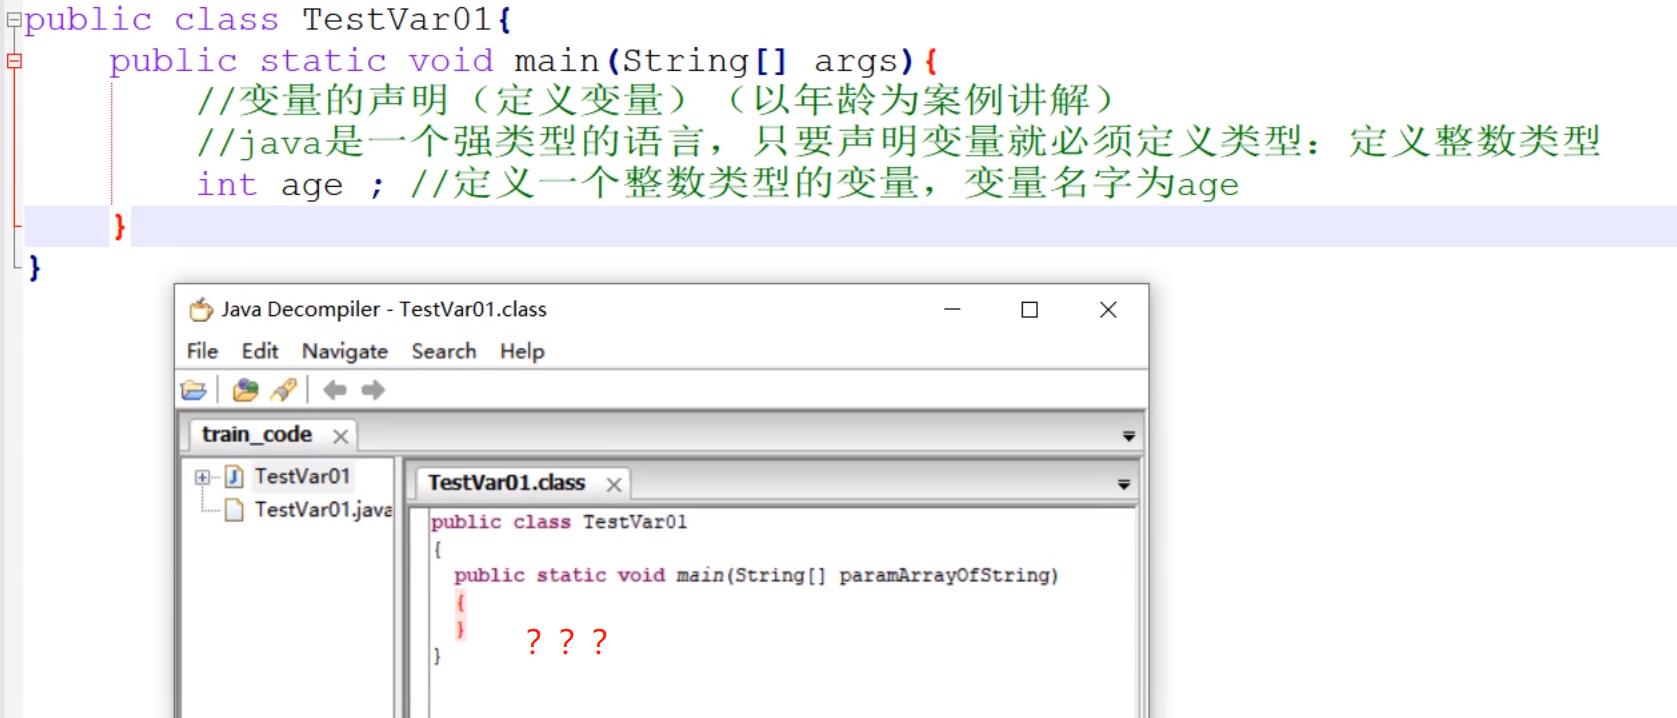
\includegraphics[width=100mm]{01.png}
	%	\caption{反编译之后的结果}
		\label{fig:label}
	\end{figure}

	line4-(System.out.println(age)):如果变量没有进行赋值的话,使用的时候会报错:尚未初始化变量,如下图所示;
	
	\begin{figure}[ht]
		\centering
		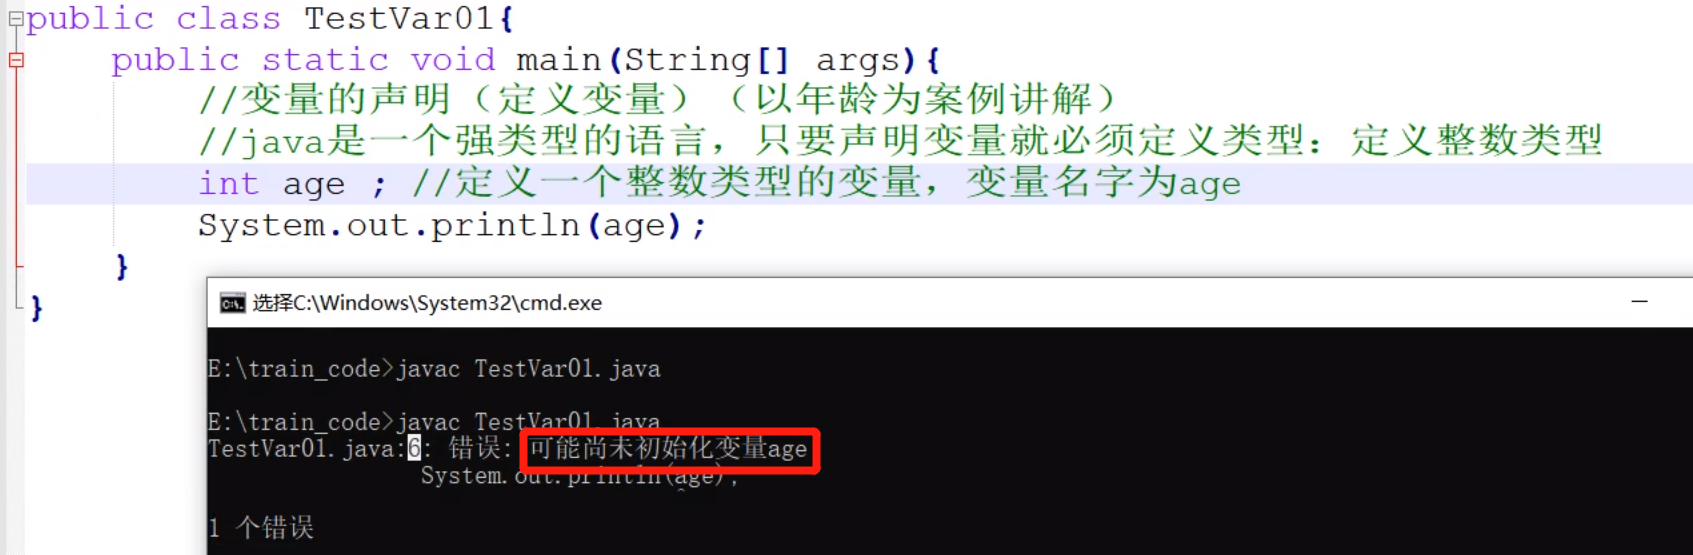
\includegraphics[width=100mm]{02.png}
	%	\caption{使用未定义的变量}
		\label{fig:label}
	\end{figure}
	
	line4:变量名字为age,具体的值为24,并且变量的值可以任意改变;
	
	%反编译:两句代码被整合为一句;变量名字变为i,如下图所示;
	
	\begin{figure}[ht]
		\centering
		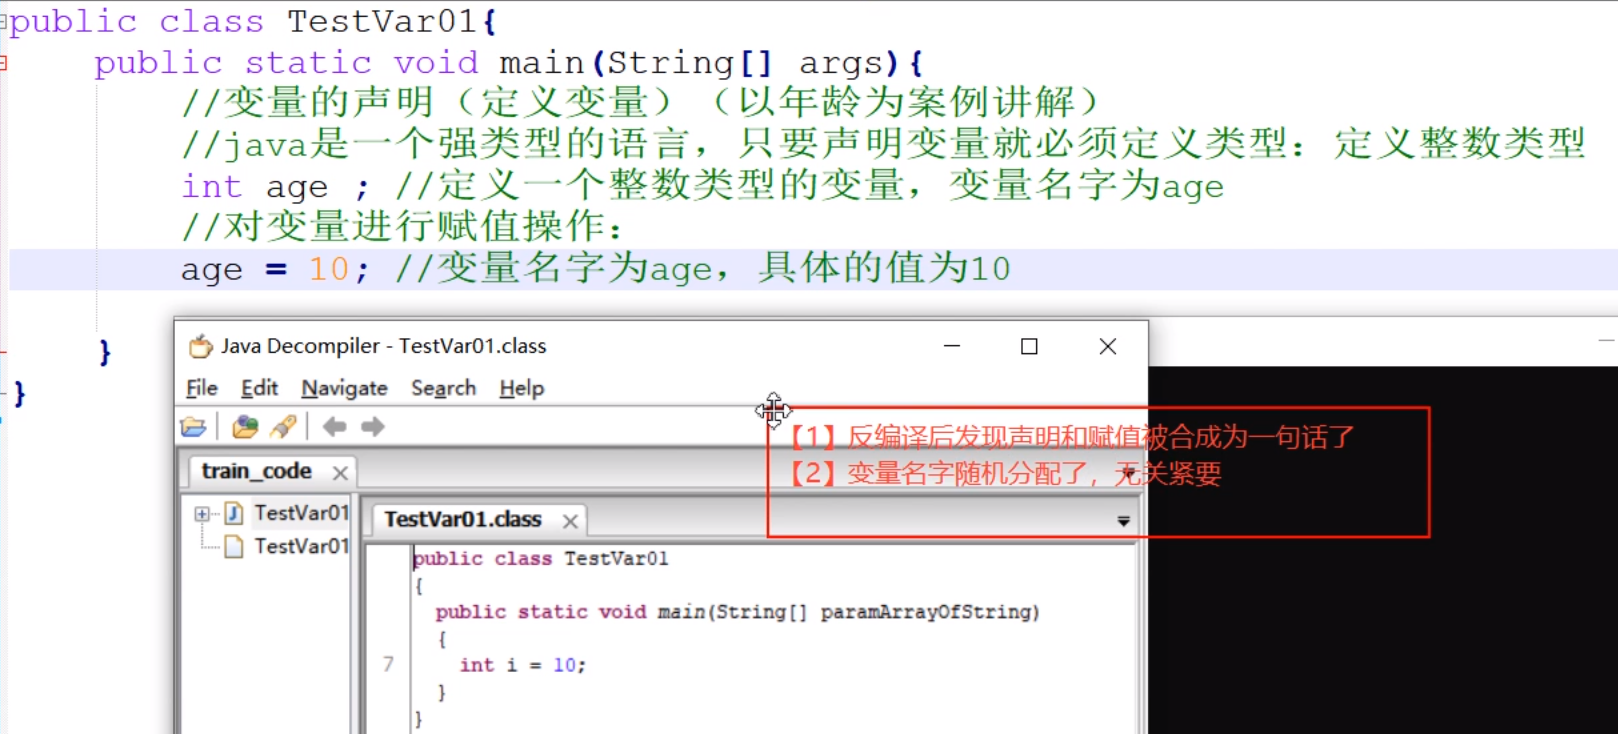
\includegraphics[width=100mm]{03.png}
	%	\caption{反编译age=24代码}
		\label{fig:label}
	\end{figure}
	
	\subsubsection{小拓展}
	
	\begin{lstlisting}
	public class TestVar02{
	    public static void main(String[] args){
	        int a=10;
	        int b=20;
	        int c=a+b;
	    }
	}
	\end{lstlisting}
	
	操作命令:javac TestVar02.java产生.class字节码文件
	
	\setlength{\parindent}{7em}javap -v TestVar02.class(-v表示verbose,查看详情,如下图)
	
	\begin{figure}[ht]
		\centering
		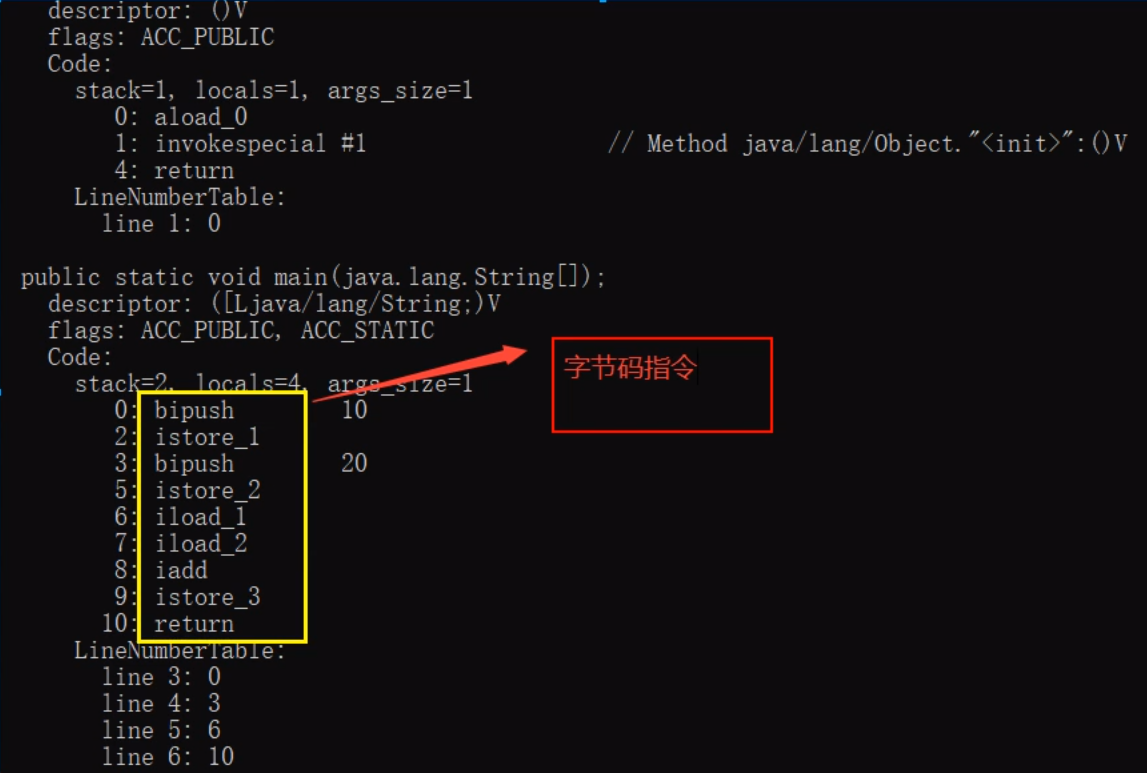
\includegraphics[width=100mm]{04.png}
		\label{fig:label}
	\end{figure}
	
	\setlength{\parindent}{2em}
	
	\subsection{变量的内存}
	
	内存只占用一块空间,以“int age=18”为例
	
	\subsection{变量的作用域}
	
	作用域指的就是作用范围,即变量在什么范围内有效(作用范围就是在定义变量之后,离变量最近的花括号)
	
	\begin{lstlisting}[ language=Java]
	public class TestVar04{
		public static void main(String[] args){
			int a = 10;
		System.out.println(a);
		}
		public void eat(){
		System.out.println(b);
		}
	}
	\end{lstlisting}
	
	备注:line4可以运行;line4复制到line3之前就不能运行,变量一定要赋值之后才有效;
	
	局部变量:定义在方法中的变量;
	
	成员变量:定义在类中但是在方法外(比如在line1和line2之间插入“int b=10;”);
	
	(那么在line4下添加一行“System.out.println(b);”是否可以访问呢?)

	(可以的,因为b是成员变量,在line1花括号到line6花括号之间,任何对b的操作都可以访问,包括line7的访问也可以;但是在line7后加“System.out.println(a);”就不能访问;但是在line7后加“int a=40;”,此动作不属于重复定义,所以可以对新定义的a进行访问)
	
	(代码块就是指一堆花括号之间的区域,出了花括号以后就不能访问;花括号之内的变量不允许再次定义,话括号内的花括号也不可以)	
	
	\subsection{基本数据类型量}
	
	Java中的数据类型有以下几种:
	
	\begin{figure}[ht]
		\centering
		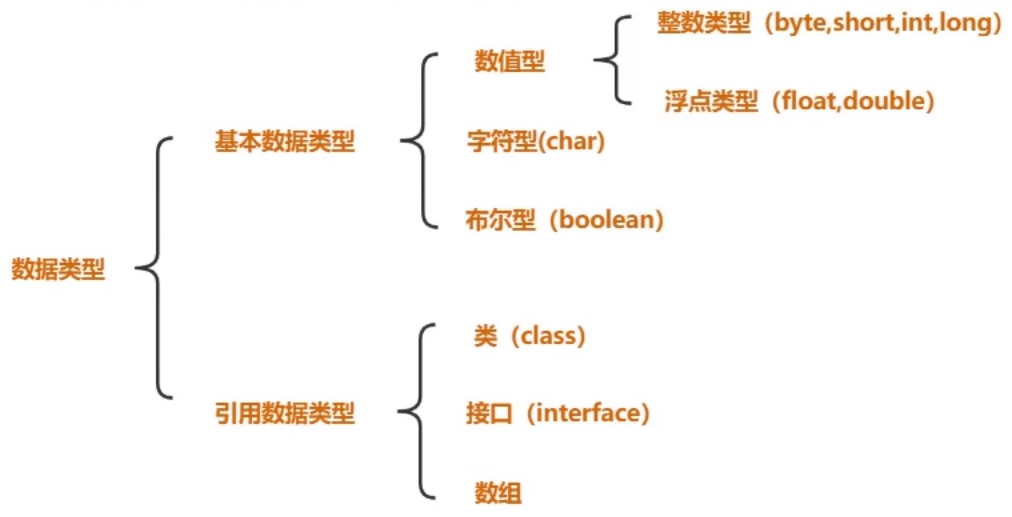
\includegraphics[width=100mm]{06.png}
		\label{fig:label}
	\end{figure}
	
	除了基本数据类型以外的所有类型,都属于引用数据类型,本章重点:基本数据类型。
	
	\subsubsection{整数类型常量}
	
	整数型常量就是数字,常见为十进制,以0开头的八进制,以0X或0x开头的十六进制,以0B或者0b开头的二进制
	(电脑系统给出的计算器就可以直接进行进制之间的转换)
	
	\subsubsection{整数类型变量}
	
	\begin{figure}[ht]
		\centering
		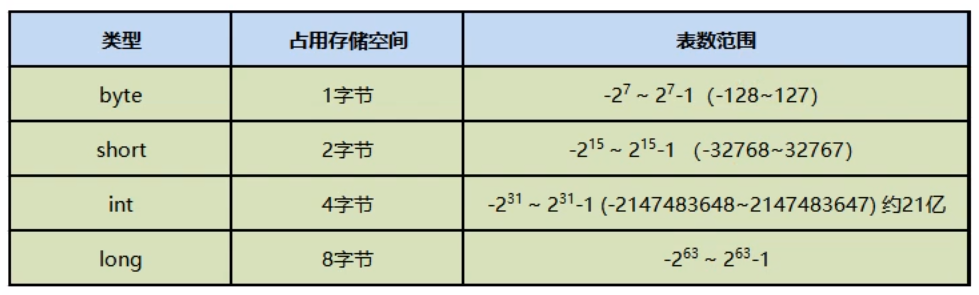
\includegraphics[width=120mm]{07.png}
		%\label{fig:label}
	\end{figure}
	
	例题:byte右侧表数范围127怎么算出来的?
	
	byte:1字节=8位0/1
	
	二进制:01111111=127(十进制)
	
\bigskip	
	
	代码:
	\begin{lstlisting}[ language=Java]
	public class TestVar04{
		public static void main(String[] args){
			int num1=12;
			System.out.println(num1);
			int num2=012;
			System.out.println(num2);
			int num3=0x12;
			System.out.println(num3);
			int num4=0b10;
			System.out.println(num4);
			byte b=12;
			System.out.println(b);
			short s=30000;
			System.out.println(s);
		}
	}
	\end{lstlisting}
	
	备注:默认情况下的赋值都是十进制的;给变量赋值的时候,可以根据不同进制进行赋值,但是最后的输出全是十进制形式。
	
	备注:“byte b=12;”定义了一个byte类型的变量,名字叫b,赋值为12,此时可以正常输出;
	
	\setlength{\parindent}{5em}“byte b=129;”属于超范围定义,会报错,因为byte类型最大只能到127;
	
	“short s=30000;”没有超范围,可以正常输出;
	
	“int i=12345678910;”达到百亿,超过了最大范围21亿,不能输出结果;
	
	“long num5=12345678910”可以实现输出;
	
	(执行的时候还是会报错,那是因为定义变量时,整数类型默认就是int类型,对于int类型来说,它超出范围了)
	
	(要想把一个长的整数赋值给long类型变量,那么在后面加上A或者L即可)
	
	\setlength{\parindent}{2em}注意:只有当这个数超出了int类型的范围后才需要加上L,fu'ze'wu'xu'guan
	
	\subsubsection{浮点类型常量}
	
	浮点就是对应的小数。
	
	182.5就是十进制下的浮点数;31415926e-7是科学计数法下的圆周率
	
	\subsubsection{浮点类型变量}
	
	float类型又称作是单精度类型,可以表示6~7位有效数字;
	
	double类型又称作是双精度类型,可以表示15~16位有效数字。
	
	float类型的数值后面默认带有后缀F或者f,没有后缀的浮点数默认为double类型,也可以加后缀D或者d以明确其确实是double类型。
	
	备注:有效数字是从左边第一个不为0的数到最后一个数。
	
	\setlength{\parindent}{5em}float4个字节32位的分配是:1符号位、2-9指数位、其余尾数位;
	
	“2乘10的4次方”中2是尾数位、10是底数、4是指数。
	
	\setlength{\parindent}{2em}
	
	\begin{lstlisting}[ language=Java]
	public class TestVar06{
		public static void main(String[] args){
		double num1=3.14;
		System.out.println(num1);
		double num1=314E-2
		System.out.println(num2);
		float f1=3.146789416513156498465;
		System.out.println(f1);
		}
	}
	\end{lstlisting}
	
	问题:编译最后是“float f1=3.146789416513156498465;”时候发生报错,显示“从Double转为float可能不兼容,会发生数据丢失”。
	
	解析:浮点型常量默认是doule类型的,要想将double类型数赋值给float类型,在最后添加F或者f。
	
	备注:doule类型之后可以加D或者d,但是一般都省略不写。
	
	注意:最好不要进行浮点类型的比较;"="表示"赋值";"=="的运算符的结果是逻辑常量,即"true"或者"false"
	
	\subsection{编码和字符集}
	
	编码:信息从一种形式变为另一种形式的过程;
	
	字符集/编码表:编码和解码过程的根据(有很多很多种类);
	
	(由权威机构形成的编码表才可以称之为字符集/编码表,如ASCII、ISO8859-1、GB2312、GBK、Unicode)
	
	ASCII是英文字符集,用一个字节的7位表示,ISO8859-1是西欧字符集,用一个字节的8位表示,GB2312和GBK分别是简体中文字符集和繁体中文字符集,最多用两个字节表示中文,so问题来了:当有两个字节分别表示英文或者西欧字符时,怎样能让计算机知道是两个字符,还是两个字节合起来是一个中文字符呢?
	
	字节第一位如果是0,则表示一个字节就足够表示该字符;如果第一位是1的话,则表示一个字节就不够表示该字符,需要和后面合起来当作一个字符来看。
	
	Unicode是国际通用字符集,融合了人类所使用的所有字符。为每个字符分配唯一的字符码。
	
	Unicode按照最多两个字节存储信息,则有2的15次方即65532种字符可以被存储,但是出现和上述一样的问题,如果第一位通过0/1进行区分一个字节还是两个字节,则可表示信息就不足以包含所有字符,于是Unicode在出现后的很长时间内都没有得以实现。
	
	直到后面互联网推出了UTF标准,它有三种编码方案:UTF-8、UTF-16、UTF-32
	
	
	
	\begin{figure}[ht]
		\centering
		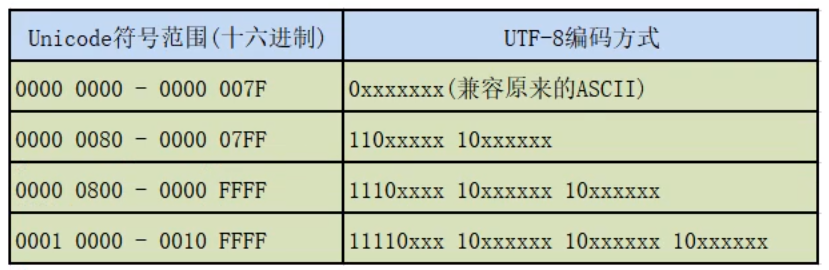
\includegraphics[width=120mm]{08.png}
		%\label{fig:label}
	\end{figure}
	
	以UTF-8为例进行讲解:中文“苗”的UTF-8码在十进制下是33495(二进制下为1000 0010 1101 0111,八进制下为101 327,十六进制下为82D7)
	
	对照上图可以看到,十六进制下的82D7落在了第三行,所以底层的二进制存储就是把“苗”的二进制码塞到第三行的框架即“1110xxxx\space\space10xxxxxx\space\space10xxxxxx”中去,得到“1110\space1000\space\space10\space001011\space\space10\space010111”
	
	(后期对UTF-8标准进行了更改,现在最多可以用6个字节表示)
	
	\subsection{字符类型}

	Java中用单引号来表示字符变量
	
	\begin{lstlisting}[ language=Java]
	public class TestVar07{
		public static void main(String[] args){
			char ch1='8';
			System.out.println(ch1);
			char ch1='a';
			System.out.println(ch2);
			char ch1='A';
			System.out.println(ch3);
			char ch1='zhongdehanzi';
			System.out.println(ch4);
			char ch1='?';
			System.out.println(ch5);
			char ch6=' ';
			System.out.println(ch6);
			System.out.println("------------------------------------");
			char ch7='\n';
			System.out.println("aaa"+ch1+"bbb");
			System.out.println("aaa \nbbb");
			System.out.println("=====================================");
			System.out.println("\"Java\"");
		}
	}		
	\end{lstlisting}
	
	转义字符:$\backslash$将后面的普通字符转换为特殊含义。
	
	备注:ch6一样也可以被输出,就算是空格,也得是单个空格;
	
		\setlength{\parindent}{5em}--------------------------------下的两句话可以理解为:上面是“字符串+字符+字符串”,下面整体是一个字符串,可以说明a+a+a成为一个字符串,$\backslash$n同样也是一个单一字符;
		
		$\backslash$t表示“需要空的格子+前面的字符串=8位”;
		
		$\backslash$b表示退格,实现过程为“输出aaa,检测到$\backslash$b后删除前一个字符,继续输出后面的bbb”;
		
		$\backslash$r的输出结果是bbb,实现过程为“输出aaa,检测到$\backslash$r之后,把光标移动到本行开头重新输出bbb”;
		
		$\backslash$"表示将"原样输出;$\backslash$'表示将'原样输出;$\backslash$$\backslash$表示将$\backslash$原样输出。
	
		\setlength{\parindent}{2em}以上代码全部都可以被运行,故Java中无论字母数字还是中文还有符号,都是字符类型的常量,都占用两个字节(char是用UTF-16标准进行编码的)
	
	\begin{lstlisting}[ language=Java]
	public class TestVar07{
		public static void main(String[] args){
		char ch1='A';
		System.out.println(ch1);
		System.out.println(ch1+90);
		System.out.println(155-ch1);
		char ch2='zhongdehanzi';
		System.out.println(ch2);
		System.out.println(ch1+90);
		System.out.println(20103-ch1);
		
		int num=(int)ch2;
		System.out.println(num);
		
		int num2='zhongdehanzi';
		char ch3=20013;
		}
	}		
	\end{lstlisting}	
	
	备注:输出结果是A,换行后155,换行后90.
	
	\setlength{\parindent}{5em}“A”→我们看到的char类型的样子就是它的字面常量本身,但是底层在进行计算的时候,实际上是按照ASCII码进行计算的。
	
	但是之前又说char类型是按照Unicode码表进行存储的,怎么解释呢?Unicode码表是兼容ASCII码表的,前128位是一样的,具体的实现过程如下图所示
	(Unicode码表网址为:https:$\backslash$$\backslash$www.cnblogs.com$\backslash$csguo$\backslash$p$\backslash$7401874.html0
	
		\begin{figure}[ht]
		\centering
		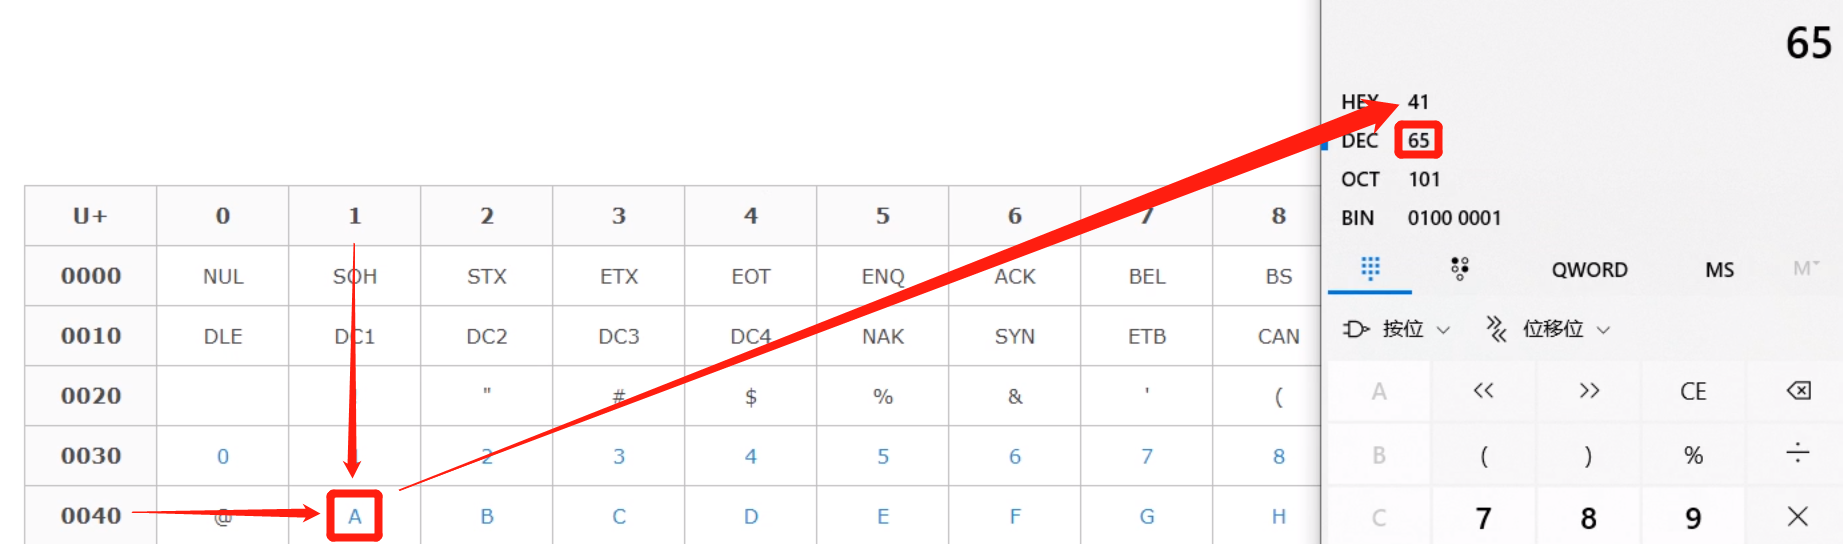
\includegraphics[width=150mm]{10.png}
		%\label{fig:label}
	\end{figure}
	
	\setlength{\parindent}{2em}小面试题:
	
	\begin{lstlisting}[ language=Java]
	public class TestVar07{
		public static void main(String[] args){
		char ch='2'+2;
		System.out.println(ch);
		}
	}		
	\end{lstlisting}	
	
	输出结果应该是4,实现过程:2对应的码为50,50参与运算,50+2=54,54在Unicode码表中对应的字符为4.
	
	\subsection{解释乱码问题}
	
	在【编码】中选择【UTF-8】后输入以下代码:
	
	\begin{lstlisting}[ language=Java]
	public class TestVar09{
		public static void main(String[] args){
			char ch1="你好 我是苗";
			System.out.println(ch1);
		}
	}		
	\end{lstlisting}	
	
	在命令控制台编译时会出现乱码是为什么呢?
	
	答:将编码格式改为UTF-8之后,表示程序中的文字是用UTF-8进行编码的,但是最终打在控制台编译时用的是GBK进行解码,所以会解成乱码。
	
	\setlength{\parindent}{4em}那么就需要将编码格式改为GBK,同时ANSI会获取当前操作系统的格式(现在的操作系统是中文的,使用的就是GBK编码格式),所以将编码格式改为ANSI后就默认使用GBK进行编码,最后命令行编译和执行代码都不会出错。
	
	备注:用记事本选择编码格式时一般要选择ANSI→获取当前系统的操作格式,一般都是GBK
		
	\setlength{\parindent}{2em}
	
	\subsection{布尔类型}
	
	Boolean类型有两个常量值,分别是true和false,在内存中占一位,不是一个字节(但是不能用0和)
	
	\begin{lstlisting}[ language=Java]
	public class TestVar10{
		public static void main(String[] args){
			boolean flag1=true;
			System.out.println(flag1);
			boolean flag2=false;
			System.out.println(flag2);
			boolean flag3=4==8;
			System.out.println(flag3);
			boolean flag4=4<8;
			System.out.println(flag4);
		}
	}		
	\end{lstlisting}
	
	备注:输出结果为“true”
	
	\subsection{基本数据类型转换问题} 
	
	输入以下代码查看输出结果:
	
	\begin{lstlisting}[ language=Java]
	
	public class TestVar10{
		public static void main(String[] args){
			double d=6;	
			System.out.println(d);
			int i=6.5;
			System.out.println(i);
			int a=(int)6.5;
			System.out.println(a);
		}
	}
	\end{lstlisting}	
	
	备注:输出结果为"6.0"$\backslash$n"从double转换到int可能会有损失"$\backslash$n"6"
	
	\bigskip
	
	什么是类型转换?
	
	在赋值运算或者算术运算的时候,要求数据类型一致,就要进行类型的转换。并且转换的种类分为自动转换(如double a=6)和强制转换(如int i=6.5,简称为强转)。
	
	在同一个表达式中,有多个数据类型的时候,应该如何处理:
	
	\begin{lstlisting}[ language=Java]
	double d=12+1256L+8.5F+3.14+'a'+true;
	\end{lstlisting}
	
	以上代码在编译的时候出错。多种数据类型参与从运算的时候,整数类型、浮点类型还有字符类型都可以参与运算,唯独布尔类型不能参与运算。
	
	\begin{lstlisting}[ language=Java]
	double d=12+1256L+8.5F+3.14+'a';
	\end{lstlisting}
	
	备注:类型级别:byte、short、char→int→long→float→double
	
	\setlength{\parindent}{5em}级别的作用:当一个表达式中有多个数据类型的时候,要找出当前表达式中级别最高的那个类型,然后其余的类型都转换为当前表达式中最高的类型进行计算。
	
	故d=12+1256L+8.5F+3.14+'a'
	
	\setlength{\parindent}{7em}=12.0+1256.0+8.5+3.14+97.0
	
	=3168.14
	
	\setlength{\parindent}{5em}在进行运算的时候,左边=右边,直接赋值;左边<右边,强制转换;左边>右边,自动转换。
	
	以下几种属于特殊情形:①对于byte、short、char类型来说,只要在他们的表述范围内,赋值时不用强转(如byte a=12不需要强转)
	
	\setlength{\parindent}{2em}
	
	\subsection{习题1——初识Scanner} 
	
	实现功能:求圆的周长和面积?
	
	\begin{lstlisting}[ language=Java]
	public class TestVar11{
		public static void main(String[] args){
			double c=2*3.14*5;	
			System.out.println("周长为:"+c);
			int s=3.14*5*5;
			System.out.println(s);
		}
	}
	\end{lstlisting}
	
	备注:输出为“周长为:31.4000000000002”,“面积为78.5”
	
	想要精度更加提高的话,$\pi$的值从3.14变化到3.1415925,但是为了避免多次输入数值,则在之前定义变量pi=3.1415926,这样就可以一劳永逸,以后只需要改变变量的值,那接下来所有用到变量的地方,也都发生变化;但是对于$\pi$这种确定的数值,不想让他人修改,则需要将程序赋值一行程序改为如下:
	
	\begin{lstlisting}[ language=Java]
	final double pi=3.1415926;	
	\end{lstlisting}
	
	如果后面对$\pi$再次进行修改的话,在编译的时候就会报错。
	
	一个变量被final修饰之后,这个变量就变成了常量,这个常量就是字符常量,其值不可以再次发生改变。
	
	(根据约定俗成的规定:字符常量的名字全部大写)
	
	\begin{lstlisting}[ language=Java]
	public class TestVar11{
		public static void main(String[] args){
			final double PI=3.1415926;
			//拿来一个扫描器:
			Scanner input=new Scanner(System.in);
			//让扫描器扫描键盘录入的int类型的数据:
			int r=input.nextInt();
			int c=2*PI*r;
			System.out.println(c);
		}
	}
	\end{lstlisting}
	
	备注:以上程序编译会报错:找不到符号Scanner(需要在第一行上面插入"import java.utill.Scanner;",可理解为在java.utill下将Scanner拿过来使用);此时编译和执行都没问题,命令控制台的光标在新的一行跳动,此时应该输入半径值并且按动回车结束;ctrl+C强制结束;为了不让光标闪烁的很突然,可以再添加"int input=sc.nextInt();"之前添加"System.out.println("请录入一个半径")"";也可以把添加的改为"System.out.print("请录入一个半径");";"int input=sc.nextInt();"表示只能输入int类型,输入其他类型会报错。
	
	\subsection{习题2——加深对Scanner的使用} 
	
	\begin{lstlisting}[ language=Java]
	import java.utill.Scanner;
	public class TestVar11{
		public static void main(String[] args){
			//键盘录入学生的信息:年龄、身高、姓名、性别:
			//键盘录入年龄:(接收int型数据)
			Scanner sc=new Scanner(System.in);
			System.out.print("请录入年龄:");//友好性提示
			int age=sc.nextInt();//"nextInt"中的System.out.prin()
			//键盘录入身高:(接收double型数据)
			System.out.print("请录入身高:");//友好性提示
			double height=sc.nextDouble();
			//键盘录入姓名:(接收string型数据)
			System.out.print("请录入姓名:");//友好性提示
			String name=sc.next();
			//键盘录入性别:(接收char类型)
			String genderStr=sc.next();
			char gender=genderStr.charAt(0);
			//以上两句可合二为一:char gender=sc.next().charAt(0);
			System.out.println("该学生的信息为:姓名是"+name+",
			年龄是"+age+",身高是"+height+",性别是"+gender);
		}
	}
	\end{lstlisting}
	
	备注:nextInt和nextDouble的"I"和"D"要大写。
	
	
	
	
\end{document}